\documentclass[../../main.tex]{subfiles}
\begin{document}

{\bf [解答]}

\begin{figure}[htb]
  \centering
  \begin{tikzpicture}[x=1.15cm, y=0.95cm, every node/.style={font=\small}]
    % A が優勝する3つのパターン（最終戦は必ず A の勝利）
    \node[anchor=east, font=\footnotesize] at (-0.2, 2.2) {\textbf{3試合}（3勝0敗）：};
    \foreach \i in {1,2} {
      \draw[thick, blue!80!black, fill=blue!10] (\i*1.15, 2.2) circle (0.26);
      \node[font=\footnotesize, blue!85!black] at (\i*1.15, 2.2) {$A$};
    }
    \draw[thick, red!80!black, fill=red!12] (4.5, 2.2) circle (0.26);
    \node[font=\footnotesize, red!85!black] at (4.5, 2.2) {$A$};
    \node[anchor=west, font=\footnotesize] at (5.05, 2.2) {確率 $p^3$};

    \node[anchor=east, font=\footnotesize] at (-0.2, 1.1) {\textbf{4試合}（3勝1敗）：};
    \draw[rounded corners=3pt, dashed, teal!80!black, fill=teal!8] (0.35, 0.72) rectangle (3.95, 1.48);
    \node[font=\footnotesize, teal!85!black] at (2.15, 1.1) {$A$ 2勝，$B$ 1勝（${}_3\mathrm{C}_1$通り）};
    \draw[thick, red!80!black, fill=red!12] (4.5, 1.1) circle (0.26);
    \node[font=\footnotesize, red!85!black] at (4.5, 1.1) {$A$};
    \node[anchor=west, font=\footnotesize] at (5.05, 1.1) {確率 $3p^2q \cdot p = 3p^3q$};

    \node[anchor=east, font=\footnotesize] at (-0.2, 0.0) {\textbf{5試合}（3勝2敗）：};
    \draw[rounded corners=3pt, dashed, teal!80!black, fill=teal!8] (0.35, -0.38) rectangle (3.95, 0.38);
    \node[font=\footnotesize, teal!85!black] at (2.15, 0.0) {$A$ 2勝，$B$ 2勝（${}_4\mathrm{C}_2$通り）};
    \draw[thick, red!80!black, fill=red!12] (4.5, 0.0) circle (0.26);
    \node[font=\footnotesize, red!85!black] at (4.5, 0.0) {$A$};
    \node[anchor=west, font=\footnotesize] at (5.05, 0.0) {確率 $6p^2q^2 \cdot p = 6p^3q^2$};
  \end{tikzpicture}
  \caption{$A$ が先に3勝して優勝する3通りの試合経過（最終戦は必ず $A$ の勝利）}
  \label{fig:1974_6_cases}
\end{figure}

題意より$A$が優勝する場合は以下のいずれかである．
\begin{align}
  \begin{cases}
    \text{$A$の$3$連勝}&p^3 \\
    \text{$A$の$3$勝$1$敗}& 3p^3q \\
    \text{$A$の$3$勝$2$敗}& 6p^3q^2
  \end{cases}\label{eq:1}
\end{align}
従って$P$が優勝する確率は
\begin{align}
  P  &=p^3*3p^3q+6p^3q^2 \nonumber\\
  &=p^3(1+3q+6q^2) \nonumber\\
  &=p^3(6p^2-15p+10)&(\because p+q=1)\label{eq:2}
\end{align}
である．同様に対称性から$Q$が優勝する確率は
\begin{align}
  Q
  &=q^3(1+3p+6p^2) \\
  &=(1-p)^3(1+3p+6p^2) \label{eq:3}
\end{align}
である．\cref{eq:2,eq:3}をまとめて
\begin{align}
  \begin{cases}
    P = p^3(6p^2-15p+10) \\
    Q = (1-p)^3(1+3p+6p^2)
  \end{cases} \label{eq:4}
\end{align}
である．

\subparagraph{(1)}

$p>q =1-p \Longleftrightarrow 1/2<p<1$のとき，$P+Q=1$に注意して，
\begin{align}
  f(p)
  &=P+Q-(p-q) \\
  &=(2P-1)-(2p-1) \\
  &=2(P-p) \\
  &=2p\left(p^2(6p^2-15p+10)-1\right) \quad (\because\text{\cref{eq:4}})\\
  &=4p\left(p-\dfrac{1}{2}\right)(p-1)(3p^2-3p-1) \label{eq:5}
\end{align}
である．$1/2<p<1$から，
\begin{align}
  \begin{cases}
    &p>0 \\
    &p-1<0 \\
    &p-\dfrac{1}{2}>0 \\
    &3p^2-3p-1<0
  \end{cases}
\end{align}
だから，$f(p)>0$すなわち
\begin{align}
  P-Q>p-q
\end{align}
である．$\cdots$(答)

\subparagraph{(2)}

前問の過程から，$f(p)=2(P-p)$を最大にする$p$を求めればよい．
\cref{eq:5}を$p$で微分して
\begin{align}
  \dfrac{1}{2}f'(p)
  &=30p^4-60p^3+30p^2-1 \\
  &=30p^2(p-1)^2-1
\end{align}
だから，$0<p<1$に注意して
\begin{align}
  f'(p)\ge0
  \Longleftrightarrow
  &p^2(p-1)^2\ge\dfrac{1}{30} \\
  \Longleftrightarrow
  &p(1-p)\ge\dfrac{\sqrt{30}}{30} \\
  \Longleftrightarrow
  &\dfrac{1}{2}\left[1-\sqrt{1-\dfrac{2\sqrt{30}}{15}}\right]
  \le p
  \le
  \dfrac{1}{2}\left[1+\sqrt{1-\dfrac{2\sqrt{30}}{15}}\right]
\end{align}
だからこれを
\begin{align}
  \alpha_{\pm} = \dfrac{1}{2}\left[1\pm\sqrt{1-\dfrac{2\sqrt{30}}{15}}\right]
\end{align}
とおくと，これは$0<p<1$の範囲にあるので，$f(p)$の増減表は以下のようになる．

\begin{table}[htb]
  \centering
  \caption{$0\le p\le 1$ における $f(p)=2(P-p)$ の増減表}
  \label{tab:1974_6_fp_variation}
  \renewcommand{\arraystretch}{1.35}
  \begin{tabular}{|c|c|c|c|c|c|c|c|}
    \hline
    $p$ & $0$ & $\cdots$ & $\alpha_{-}$ & $\cdots$ & $\alpha_{+}$ & $\cdots$ & $1$ \\
    \hline
    $f'(p)$ & $-2$ & $-$ & $0$ & $+$ & $0$ & $-$ & $-2$ \\
    \hline
    $f(p)$ & $0$ & $\searrow$ & 極小 & $\nearrow$ & 極大 & $\searrow$ & $0$ \\
    \hline
  \end{tabular}
\end{table}

従って $f(p)$ を最大にするのは$p=0$または$p=\alpha_{+}$である．
\cref{eq:5}から
\begin{align}
  f(0)=0
\end{align}
であり，また$\dfrac{1}{2}<p$の時$f(p)>0$であって，
\begin{align}
  \alpha_{+} = \dfrac{1}{2}\left(1+\sqrt{1-\dfrac{2}{15}\sqrt{30}}\right)>\dfrac{1}{2}
\end{align}
だから$f(\alpha_{+})>f(0)$が従う．

以上から$f(\alpha_{+})>f(0)$なので求める$p$の値は
\begin{align}
  p=\alpha_{+}=\dfrac{1}{2}\left(1+\sqrt{1-\dfrac{2}{15}\sqrt{30}}\right)
\end{align}
である．$\cdots$(答)

\subparagraph{(3)}

試合数は$3,4,5$回のいずれかであって，それぞれ$p$, $q$が勝つ場合の両方があるから
\begin{align}
  \begin{cases}
    \text{試合数 $3$回}& p^3+q^3 \\
    \text{試合数 $4$回}& 3p^3q + 3q^3p\\
    \text{試合数 $5$回}& 6p^3q^2 + 6q^3p^2
  \end{cases}\label{eq:6}
\end{align}
である．従って$N$の期待値を$N(p)$とすると:
\begin{align}
  N(p)
  &= 3(p^3+q^3)+4(3p^3q+3pq^3)+5(6p^3q^2+6p^2q^3) \\
  &= 3(p^3+q^3)+12pq(p^2+q^2)+30p^2q^2(p+q)
\end{align}
となる．$p+q=1$に注意して $t=pq$ とおいて変形すると
\begin{align}
  N(p)
  &=3(p^3+q^3)+12pq(p^2+q^2)+30p^2q^2 \\
  &=3\left[(p+q)^3-3p^2q-3pq^2\right] + 12pq\left[(p+q)^2-2pq\right] + 30p^2q^2 \\
  &=3(1-3pq) + 12pq(1-2pq) + 30p^2q^2 \\
  &=3(1-3t)+12t(1-2t)+30t^2 \\
  &=3+3t+6t^2
\end{align}
である．

\begin{figure}[htb]
  \centering
  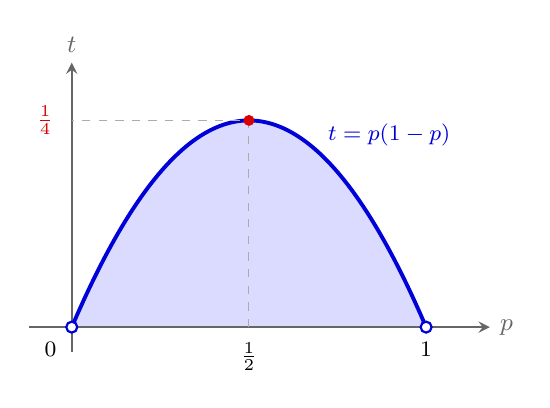
\begin{tikzpicture}[x=4.5cm, y=10.5cm, >=stealth, every node/.style={font=\small}]
    % Graph of t = p(1-p) for 0 < p < 1
    \fill[blue!14] (0, 0)
    -- plot[domain=0:1, samples=80] (\x, {\x*(1-\x)})
    -- (1, 0) -- cycle;

    \draw[->, thick, gray!80!black] (-0.12, 0) -- (1.18, 0) node[right] {$p$};
    \draw[->, thick, gray!80!black] (0, -0.03) -- (0, 0.32) node[above] {$t$};

    \draw[line width=1.4pt, blue!85!black, domain=0:1, samples=80, smooth]
    plot (\x, {\x*(1-\x)});

    \draw[dashed, gray!65] (0.5, 0) -- (0.5, 0.25) -- (0, 0.25);

    \node[circle, fill=red!85!black, inner sep=1.4pt] at (0.5, 0.25) {};
    \node[circle, draw=blue!85!black, thick, fill=white, inner sep=1.4pt] at (0, 0) {};
    \node[circle, draw=blue!85!black, thick, fill=white, inner sep=1.4pt] at (1, 0) {};

    \node[below left=2pt, font=\footnotesize] at (0, 0) {$0$};
    \node[below=2pt, font=\footnotesize] at (0.5, 0) {$\frac{1}{2}$};
    \node[below=2pt, font=\footnotesize] at (1, 0) {$1$};
    \node[left=3pt, font=\footnotesize, red!85!black] at (0, 0.25) {$\frac{1}{4}$};
    \node[above right=2pt, font=\footnotesize, blue!85!black] at (0.68, 0.20) {$t=p(1-p)$};
  \end{tikzpicture}
  \caption{$0<p<1$ における $t=p(1-p)$ のグラフ（$p=\dfrac{1}{2}$ で最大値 $t=\dfrac{1}{4}$）}
  \label{fig:1974_6_tp_graph}
\end{figure}

$t=p(1-p)$は$0<p<1$の範囲で正であり，
この範囲で$N(p)$は$t$について単調増加である．
またAM-GMから
\begin{align}
  t=p(1-p)\le\dfrac{1}{4} \quad (\text{等号成立は$p=1/2$})
\end{align}
であるから，$N(p)$は$p=\dfrac{1}{2}$で最大値$\dfrac{33}{8}$をとる．$\cdots$(答)

\newpage
\end{document}
